% Queued after the introduction so this two-column float appears on page 3.
\begin{figure*}[!t]
    \centering
    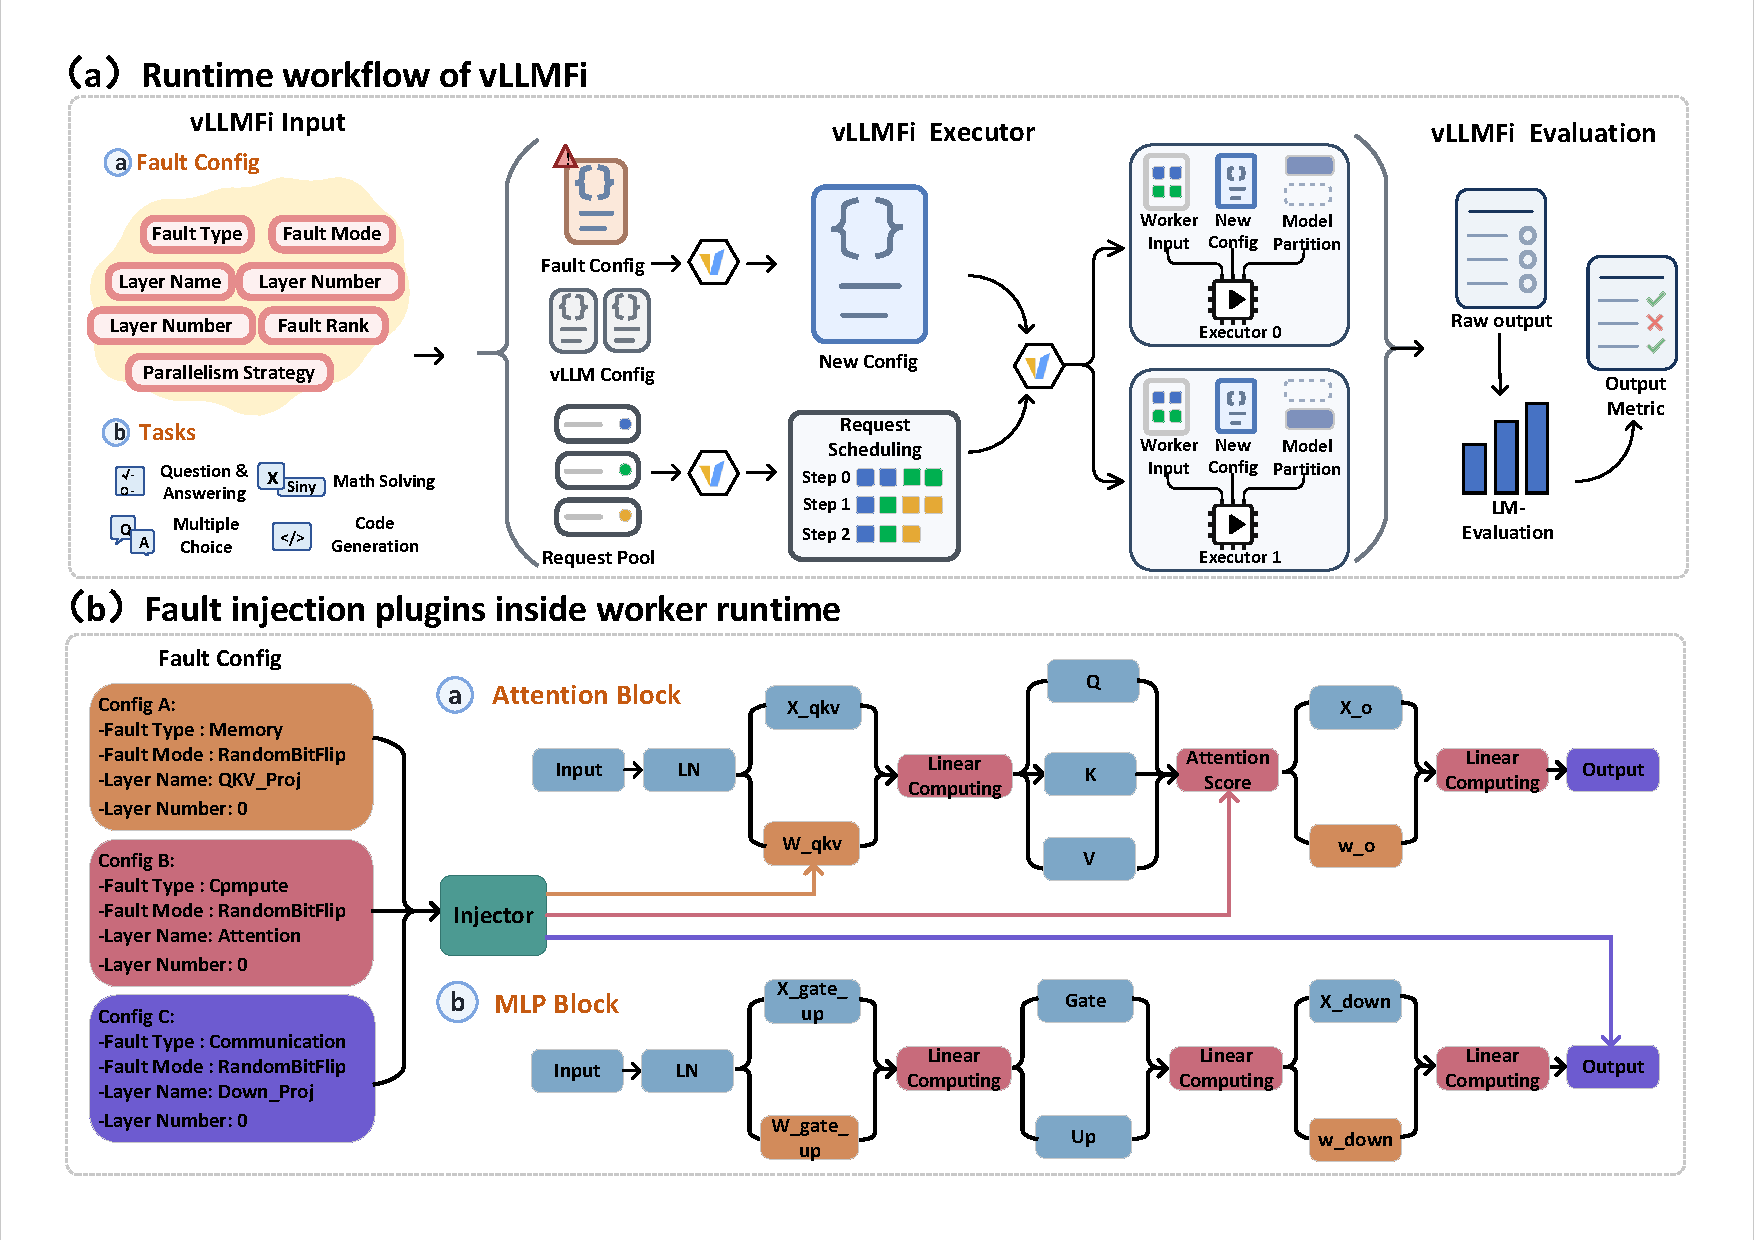
\includegraphics[
        width=\textwidth,
        trim=6pt 4pt 6pt 4pt,
        clip
    ]{vLLMFI.pdf}
    \caption{\textbf{Overview of vLLM-FI.}
    (a) Overall workflow: fault configuration and task inputs, distributed execution through the vLLM-FI executor, and task-level scoring through vLLM-FI evaluation.
    (b) Injection locations within Worker-side model computation, illustrated by QKV projection weights, an attention-computation result, and the MLP down-projection output buffer for memory, compute, and communication faults, respectively.}
    \label{fig:vllmfi_architecture}
\end{figure*}